\documentclass[titlepage]{scrartcl}
% Code Darstellung
\usepackage{listings}
\usepackage{listingsutf8}
\usepackage{multicol}

%lange Tabellen
\usepackage{longtable}
%Referenzen zwischen unterschiedlichen Dateien
\usepackage{xr}
%\externaldocument{theorie}
\usepackage{lscape}
%Deutsche Sprachunterstützung
\usepackage[utf8]{inputenc}
\usepackage[ngerman]{babel}
\usepackage{marvosym}
\DeclareUnicodeCharacter{20AC}{\EUR}

%Für das Einbinden von Bildern
\usepackage{graphicx}

%Tabellen
\usepackage{array}

%Tabellen automatisch schoener
\usepackage{booktabs}

%Caption
\usepackage{caption}
\usepackage{subcaption}

%Formeln
\usepackage{mathtools}
\usepackage{amsmath}
\usepackage{amssymb}
\usepackage{amstext}
\usepackage{dsfont}

%\usepackage{mnsymbol}

% Interssante natbib Optionen: 
% numbers : Nummerierte Zitateinheiten
% sort&compress : Bei mehrfachen Zitaten, Sortierung und ggf. Verkürzungen
%\usepackage[]{natbib}

%Vectorpfeile schöner
\usepackage{esvect}

%Formatierung
\usepackage[T1]{fontenc}
\usepackage{lmodern}
\usepackage{microtype}

%Schaltbilder malen
%\usepackage[europeanresistors,cuteinductors,siunitx]{circuitikz}
\usepackage{comment}
\usepackage{csquotes}

%Formatierungsanweisungen
\newcommand{\wichtig}[1]{\underline{\large{#1}}}
\newcommand{\aref}[1]{Abb. \ref{#1}}
\newcommand{\R}{\mathbb{R}}
\newcommand{\K}{\mathbb{K}}
\newcommand{\C}{\mathbb{C}}
\newcommand{\mr}[1]{\mathrm{#1}}

%Klickbare Referenzen
%\usepackage[hidelinks]{hyperref}
%\includeonly{theorie}
%\includeonly{theorie,versuchsdurchfuehrung,ergebnisse,anhang}
\begin{document}

\title{Spektroskopie}
\subtitle{Gruppe 1}
\date{März 2014}
\author{Udo Beier \and Leon Brückner \and Valentin Olpp \and Sebastian Ziegler}

\maketitle
\tableofcontents
\newpage
\listoffigures
\listoftables
\newpage
\section{Abstract}
\section{Einleitung}
Bereits in der Schule lernt man, dass Licht aus verschiedenen Farben zusammengesetzt ist. Dies zeigt sich z.B. bei Prismen oder am natürlichen Phänomen des Regenbogens. 1814 hat Joseph von Fraunhofer im Sonnenspektrum schwarze Linien entdeckt.\footnote{\ \cite{ktroskopie}} Er konnte den Ursprung der nach ihm benannten Linien jedoch nicht erklären. Heutzutage ist der Ursprung der Linien bekannt. Die Linien entstehen dadurch, dass die Atome der Sonne nur das Licht bestimmter Frequenzen absorbieren können, was es erlaubt, aus Absorptions- oder Emissionsspektren von Licht auf Eigenschaften der Lichtquelle zu schließen. Das Zerlegen und Analysieren von Spektren wird als Spektroskopie bezeichnet und erlaubt die Erforschung vieler Eigenschaften von Himmelskörpern, wie z.B. die Bestimmung von Radialgeschwindigkeiten oder die Spektralklassifikation von Sternen. Im Folgenden wird sich deshalb mit der Spektroskopie beschäftigt.

%Quelle:   http://de.wikipedia.org/wiki/Spektroskopie

Für den elektromagnetischen Feldstärketensor gilt:
\begin{equation}
F^{\mu \nu} = \partial^{\mu} A^{\nu} - \partial^{\nu} A^{\mu}
\end{equation}
Dabei ist A das 4er-Verktorpotential.
Dies wird als Grundwissen vorausgesetzt und hier deshalb nicht weiter vertieft.
\section{Methoden}
\subsection{Zeitmaße}

Es existieren verschiedene Zeitmaße mit unterschiedlichen Definitionen, die im folgenden aufgeführt sind.
\begin{itemize}
\item Wahre Sonnenzeit (WZ): Die wahre Sonnenzeit wird am Stand der Sonne am Himmel gemessen und beträgt 12 Uhr, wenn die Sonne durch den Meridian des Standortes geht.
\item Mittlere Sonnenzeit (MZ): Die mittlere Sonnenzeit ist eine kurzfristig gleichmäßig vergehende Zeit, wobei eine fiktive mittlere Sonne den Zeitverlauf bestimmt. Sie läuft längs des Äquators
\item Weltzeit, Universal Time (UT): Die Weltzeit ist ein Zeitmaß, das aufgrund internationaler Vereinbarungen für jeden Ort die gleiche Zeit liefert. Sie entspricht dabei der mittleren Sonnenzeit auf dem 0-Meridian.
\item Zonenzeit: Als Zonenzeit wird eine einheitliche Zeit innerhalb einer Zeitzone bezeichnet. Dabei wird die Erde in 24 Zeitzonen eingeteilt, um innerhalb einer Zeitzone vertretbare Abweichungen von der mittleren Sonnenzeit zu gewährleisten.
\item Julianisches Datum (JD): Das Julianische Datum gibt die Tage an, die seit dem 1. Januar -4712, 12 Uhr vergangen sind.
\item Sternzeit, Sidereal Time (ST): Die Sternzeit ist ein Zeitmaß, das auf der scheinbaren Rotation der Sterne am Himmel, hervorgerufen durch die Erdrotation, beruht. Ein Sterntag ist die Dauer, die der Sternenhimmel für ein ganze scheinbare Umdrehung benötigt. Die ST definiert sich als Stundenwinkel des Frühlingspunkts.
\item Ephemeridenzeit (ET,TT oder TDT): Die Ephemeridenzeit ist ein durch die Dynamik des Sonnensystems definiertes Zeitmaß. Eine Ephemeridensekunde entspricht dabei dem 31.556.925,9747ten Teil des Tropischen Jahres 1900. 
\item Atomzeit: Die Atomzeit ist ein Zeitmaß das auf der SI-Sekunde basiert und wird weltweit bei zahlreichen Zeitinstituten in der Regel durch Cäsium-Atomuhren realisiert. Eine Sekunde ist das 9.192.631.770-fache der Periodendauer der dem Übergang zwischen den beiden Hyperfeinstrukturniveaus des Grundzustandes von Atomen des Nuklids Cs-133 entsprechenden Strahlung.
\end{itemize}

Dabei verlaufen die Ephemeridenzeit und die Atomzeit streng gleichförmig, ungleichmäßig dagegen verlaufen die mittlere Sonnenzeit, die Weltzeit und die Zonenzeit aufgrund der Schwankungen der Erdrotation.

Die wahre Sonnenzeit verläuft aus zwei Gründen ungleichmäßig: Zum einen wird der gleichmäßige Verlauf durch die elliptische Form der Erdbahn und zum anderen durch die Neigung der Erdachse gestört.

Die Sternzeit steht unter dem Einfluss von Schwankungen der Rotation der Erde, wie z.B. die Präzession. Daher verläuft die Sternzeit nicht streng gleichförmig.

\subsection{Astronomische Koordinatensysteme}
Für diese Messung sind drei Koordinatensysteme von besonderer Bedeutung.

\subsubsection{Horizontsystem}

Der Ursprung des Horizontsystems liegt beim Beobachter, der Grundkreis ist der lokale Horizont. Längen- und Breitenkoordinaten entsprechen Höhenwinkel und Azimut. Die Pole sind Zenit und Nadir, wesentlicher Verwendungszweck sind Messungen an der Erdoberfläche. 

\subsubsection{Festes Äquatorsystem}

Beim festen Äquatorialsystem liegt der Ursprung wahlweise im Beobachter oder im Erdmittelpunkt. Der Grundgkreis ist hier der Himmeläquator, Längen- und Breitengrad entsprechen Deklinations- und Stundenwinkel. Die Pole sind die Himmelspole selbst. Verwendet wird dieses System vor allem bei astronomischen Beobachtungen. 

\subsubsection{Bewegliches Äquatorsystem}

Das bewegliche Äquatorialsystem entspricht dem festen, bis auf den Unterschied, dass Längen- und Breitengrad Deklinationswinkel und Rektazension entspricht. 

\subsection{Azimut und Deklination}
In einem Koordinatensystem mit einer Grundebene, welche im Fall etwa des Horizontsystems die Erdoberfläche ist, und einem dazu senkrechten Zenit, definiert man die Deklination als den Winkel zwischen Objekt und der Grundebene, sowie den Azimut als Winkel relativ zu einer ausgezeichneten Richtung. Im Fall des Horizontsystems ist dies etwa die Nord-Süd-Richtung, wobei 0 $^\circ$ Süden entspricht und die Zählung über Westen, Norden und Osten fortgesetzt wird.  

\subsection{Der Theodolit}
Für die Bestimmung der relativen Azimutwerte wird ein Theodolit verwendet, welcher mittels einer Montierung auf den Teleskopsäulen im Garten befestigt werden kann. An der Montierung wird ein Element in Form eines regelmäßigen Dreiecks befestigt, das mittels zweier Feinhorizontierschrauben relativ zur Montierung bewegt werden kann, allerdings nur um sehr kleine Wege. Dieser Mechanismus dient der Feineinstellung. Der Rest des Theodoliten ist mit einem Kugelgelenk mit dem vorherigen Element verbunden. \\
Daran schließt sich der eigentliche Theodolit an: Dieser ist zum einen drehbar um die vertikale Achse, zum anderen drehbar um eine horizontale Achse gelagert, sodass nun jeder beliebige Punkt am Himmel durch das sich anschließende Fernrohr anvisiert werden kann.  Des weiteren existiert eine Einrichtung zur Einstellung des Nullpunktes der Azimut-Skala sowie eine Wasserwaage, mit der die horizontale Ausrichtung des Theodoliten geschieht. \\
Im ersten Schritt soll der Theodolit horizontal ausgerichtet werden, sodass sich also bei einer Drehung des Theodoliten um die vertikale Achse nur der Azimut des betrachteten Objekts ändert und nicht dessen Deklination.\\
Dazu wird zunächst der Theodolit mittels des Kugelgelenks und einer Libelle (kreisförmige \enquote{Wasserwaage}) grob horizontal ausgerichtet. Die Feinjustierung geschieht dann mittels eines Algorithmus, mit dem man sich der horizontalen Ausrichtung annähert: Zunächst wird die Wasserwaage entlang einer Seite der dreieckigen Grundfläche ausgerichtet und die Ausrichtung des Theodoliten mit der entsprechenden Feinhorizontierschraube exakt auf Null eingestellt. Danach wird der Theodolit um 180 $^\circ$ um die vertikale Achse gedreht und der neue Ausschlag der Luftblase mittels der gleichen Feinjustierschraube halbiert. Anschließend wird der Theodolit um selbige Achse nochmals um 90 $^\circ$ gedreht und der Ausschlag der Luftblase mit der zweiten Feinhorizontierschraube auf den vorherigen Spielpunkt eingestellt. Indem dieses Vorgehen wiederholt wird, erreicht man nach ausreichend vielen Wiederholungen eine hinreichend genaue horizontale Justierung des Theodoliten. \\

\subsection{Messungen mit dem Theodoliten}
Azimut und Deklination eines Objekts können bestimmt werden, indem das entsprechende Objekt anvisiert wird. Durch Umlegen eines Schalters kann man zwischen Deklination und Azimut wechseln. Der entsprechende Wert kann dann durch das Mikroskoprändel angelesen werden. Dazu muss die Mikrometertrommel derart eingestellt werden, dass die Lücken in den beiden sichtbaren Balken exakt nebeneinander liegen. 

\subsection{Messung des Turmazimuts}
Mit einem derart justierten Theodoliten können nun Azimut und Deklination eines Objekts am Himmel bestimmt werden, indem man das entsprechende Objekt anvisiert und auf der Skala nun den jeweiligen Winkel, der in gon angezeigt wird, abliest. Dabei kann die Deklination als absoluter Wert im Horizontsystem abgelesen werden, wohingegen der Azimut nur relativ zu einem frei einstellbaren Nullpunkt bestimmbar ist. \\
Um nun den Azimut des angesprochenen Objekts zu bestimmen, wird nun der relative Azimut des Objekts sowie der Azimut eines anderen Objekts abgelesen, der beispielsweise mittels Literatur- und Tabellenwerten als absoluter Wert bestimmt werden kann. Dieses zweite Objekt ist in diesem Fall die Sonne. \\
Um den Turmazimut zu bestimmen, wird das Objekt mittels des Fadenkreuzes derart anvisiert, dass sich die Turmspitze möglichst exakt zentral im Fadenkreuz befindet. \\

\subsection{Messung des Sonnenazimuts}
Da die Sonne nicht direkt durch das Fernrohr beobachtet werden kann, da dies zu einer sofortigen Schädigung des Auges und der Sehfähigkeit führen würde, muss hierfür ein Filter verwendet werden. Bei der Messung wurden eine Kombination aus einem UV-IR-Rejection-Filter sowie aus zwei Neutraldichte-Filtern mit den Werten 1.8 und 3.0 eingesetzt. \\ 
Zur Bestimmung des Sonnenazimuts wird ein Überstreichen der Sonnenscheibe über einen senkrechten Strich des Fadenkreuzes betrachtet. Mit einer Stoppuhr wird eine Zeitmessung gestartet, wenn der rechte Rand der Sonnenscheibe jenen Strich berührt. Wenn der linke Rand den gleichen Strich überstreicht, wird eine Zwischenzeit genommen, zu einem frei gewählten Zeitpunkt, der ebenfalls notiert wird, wird schließlich die Messung beendet. Aus diesen drei Messungen kann der Zeitpunkt in MEZ bestimmt werden, an dem das Zentrum der Sonnenscheibe das Zentrum des Fadenkreuzes überstreicht. Der Zeitpunkt, zu dem das Zentrum der Sonne das Zentrum des Fadenkreuz überstreicht, kann einfach mittels der folgenden Formel bestimmt werden: 
\begin{equation}
U_{zen} = U_{end} - (t_{end} - \frac {t_{zw}}{2}), 
\end{equation}
wobei $U_{zen}$ die Uhrzeit des Zentrumdurchgangs, $U_{end}$ die Uhrzeit bei Beendigung der Messung, $t_{end}$ die von der Stoppuhr am Ende der Messung angezeigte Zeit sowie $t_{zw}$ die gemessene Zwischenzeit auf der Stoppuhr. 

\subsection{Berechnung des absoluten Sonnenazimuts}
Mittels der in ... dargestellen Berechnung kann aus Tabellenwerten für die Sternzeit um 0 Uhr des Messtages in Greenwich, den aktuellen Offset zwischen universal time (UT) und Ephemeridenzeit (TT) sowie den Werten für die Sonnendeklination und den Sonnenazimut im Äquatorialsystem zu Beginn und Ende des Messtages der absolute Azimut der Sonne zu jedem Messzeitpunkt eines Wertes für den Sonnenazimut bestimmt werden. Daraus ergibt sich durch Mittelung der Offset zwischen dem eingestellten Nullpunkt des Azimuts und der Nord-Süd-Verbindung. 
Durch Addition des Unterschiedes zwischen den relativen Azimutwerten für Turm und Sonne kann so der absolute Azimut des Turms bestimmt werden. 
\section{Auswertung}
\subsection{Bestimmung der Auflösung}
Aus dem aufgenommenen Spektrum der ThAr-Lampe kann empirisch eine Auflösung bestimmt werden, indem für mehrere Linien der Quotient aus Wellenlänge und Halbwertsbreite bestimmt und gemittelt wird. Dies wurde in MIDAS durchgeführt, indem über die Peaks eine Gaußfunktion gefittet wurde. Die erhaltenen Daten sind in Tabelle \ref{tab:Aufloesung}, Seite  \pageref{tab:Aufloesung} enthalten. Der Wert wurde also über die Formel
\begin{equation}
R_{Emp} = \frac{\lambda}{b}
\end{equation}
bestimmt, wobei $\lambda$ die Wellenlänge und $b$ die Halbwertsbreite ist. Der aus diesen Werten bestimmte Mittelwert mit Standardabweichung ergibt sich zu:
\begin{equation}
R_{Emp} = 13663.3 \pm 2445.8
\end{equation}
Dieser Wert lässt sich auch von MIDAS direkt berechnen, wobei MIDAS das Ergebnis
\begin{equation}
R_{Emp} = 12547.7 \pm 3398.3
\end{equation}
ausgibt. Es ist anzunehmen, dass MIDAS eine weitaus größere Anzahl von Linien für die Berechnung des Werts verwendet, deswegen ist dieser Wert trotz der größeren Standardabweichung als genauer anzunehmen.
\\
Es wurden bereits aus theoretischen Überlegungen Auflösungen für das Spektrometer und die CCD-Kamera bestimmt:
\begin{equation}
R_{Echelle} = 24416
\end{equation}
\begin{equation}
R_{CCD} =  25000
\end{equation}
Man sieht, dass die empirisch bestimmte Auflösung zwar in der gleichen Größenordnung, aber um ca. einen Faktor 2 kleiner ist.\
Dies ist vor allem dadurch begründet, dass die Kollimatorlinse nicht \enquote{perfekt} ist, also verschiedene Wellenlängen unterschiedlich stark bricht. Dadurch verändert sich die Brennweite der Linse je nach Wellenlänge und das Bild wird unscharf. Eine Verbesserung der tatsächlichen Auflösung wäre also nur durch eine bessere, d.h. farbtreuere Linse möglich, dies würde aber die Kosten für den Spektrographen entsprechend hochtreiben.

\subsection{Auswertung der Spektren}
\subsubsection{Die Harvard-Klassifikation}
Die folgenden Informationen wurden entnommen aus \cite{ttunen}:\\
Sterne können anhand ihres Spektrums in verschiedene Typen eingeteilt werden. Diese Einteilung heißt Harvard-Klassifikation und ordnet Sterne in die Klassen O,B,A,F,G,K, oder M ein (fränkischer, geschlechtsneutraler Merkspruch: \enquote{Ohne Bier ausm Fass gibts ka Maß}). Eine Einteilung der Sterne in diese Klassen ist anhand des Vorhandenseins bestimmter Absorptionslinien möglich. Der Unterschied zwischen Spektren von verschiedenen Sternen ist vor allem durch die Temperatur der Sterne bedingt. Die Linien werden durch Absorption von Photonen durch die Elektronen der Atome in der stellaren Atmosphäre erzeugt. So wird z.B. die Helium I - Linie durch Absorption von Photonen durch He-Atome im angeregten Zustand erzeugt. Der Übergang vom Grundzustand in den angeregten Zustand ist durch Photonen aus dem sichtbaren Spektrum nicht möglich. Um die He-Atome anzuregen, muss die Temperatur aber entsprechend hoch sein, sodass diese Linie in kalten Sternen nicht zu sehen ist. Bei höherer Temperatur sind auch mehr Atome im angeregten Zustand, womit mehr Photonen absorbiert werden und die Linie eine stärkere (bzw. niedrigere) Intensität erhält. Wenn die Temperatur weiter ansteigt, werden die He-Atome jedoch ionisiert und können daher keine Photonen mehr absorbieren, womit die Intensität der Linie wieder abnimmt (bzw. größer wird). Mit diesen Mechanismen lässt sich auch das Verhalten anderer Linien (Ca I, He II, Fe I) erklären. Bei Molekülen (z.B. TiO) gibt es so viele Übergänge, dass sie im Spektrum nicht mehr unterschieden werden können und als durchgängiges Absorptionsband erscheinen. Eine graphische Übersicht ist in Abb. \ref{fig:Harvard} dargestellt.
\\
Anhand der Absorptionslinien im Spektrum kann man nun einige Kriterien zur Einteilung angeben:
\begin{itemize}
\item Wenn das Spektrum nur wenige, dafür sehr intensive Linien zeigt, ist der Stern heiß, also in den Klassen O, B oder A.
\item Wenn das Spektrum sehr viele Linien zeigt, ist der Stern kalt, also in den Klassen F, G, K oder M.
\end{itemize}

Kalte Sterne zeigen viele Linien in ihrem Spektrum, da Elemente wie Eisen oder Calcium nur wenig Energie für die Übergänge zwischen Energieniveaus benötigen und aufgrund der großen Anzahl von Elektronen auch viele Übergänge besitzen. Bei heißen Sternen sind diese Atome bereits ionisiert und es dominieren die Übergänge von Wasserstoff und Helium.

\begin{table}
\centering
\begin{tabular}{c|c|c|c|c|c|c}

 & He II & He I & Fe II & Ca I & G-Band & TiO-Band \\ 
\hline 
O & $\bullet$ & $\bullet$ &  &  &  &  \\ 
\hline 
B &  & $\bullet$ &  &  &  &  \\ 
\hline 
A &  &  &  &  &  &  \\ 
\hline 
F &  &  & $\bullet$ &  &  & \\ 
\hline
G &  &  &  & $\bullet$ & $\bullet$ &  \\ 
\hline 
K &  &  &  & $\bullet$ &  &  \\ 
\hline 
M &  &  &  & $\bullet$ &  & $\bullet$ \\ 
\end{tabular}
\caption{Existenz von Absorptionslinien nach Spektralklasse}
\label{tab:Spektralklassen}
\end{table}

\begin{figure}
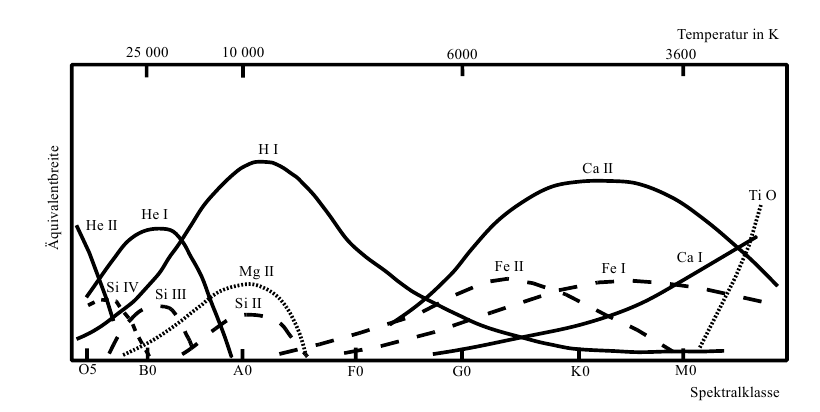
\includegraphics[width=1\textwidth]{images/Spektralklassen.png}
\caption{Qualitative Abhängigkeit der Äquivalentbreite einiger Elemente von der Spektralklasse/Temperatur eines Sternes (Abbildung entnommen aus \cite{ronomischesPraktikum})}
\label{fig:Harvard}
\end{figure}

Mit diesen beiden Kriterien und den in Tabelle \ref{tab:Spektralklassen} dargestellten Linien kann man Sterne sehr gut anhand ihres Spektrums in Spektraltypen einordnen. Da die Übergänge zwischen Spektraltypen fließend sind, ist die so gefundene Einordnung aber manchmal nicht eindeutig und es muss eine gründlichere Untersuchung durchgeführt werden, für die Zwecke des Praktikums ist dies aber ausreichend.

\subsubsection{Untersuchung des Sonnenspektrums}
In dem reduzierten aufgenommenen Sonnenspektrum wurden die wichtigsten Absorptionslinien (entnommen aus \cite{ronomischesPraktikum}) identifiziert und deren Position in MIDAS mittels einer gefitteten Gaußfunktion bestimmt. Die Abweichungen von den theoretischen Werten wurden bestimmt und daraus ein Mittelwert mit Standardabweichung berechnet. Die Werte sind in Tabelle \ref{tab:Sonne}, Seite \pageref{tab:Sonne} aufgetragen.\
Die Verschiebung von Spektrallinien ist durch den Dopplereffekt bedingt, der bei sich relativ zum Empfänger bewegenden Licht- bzw. allgemeinen Quellen auftritt. Da die Sonne jedoch relativ zur Erde keine Radialgeschwindigkeit besitzt, weil die Erde sich in einer Kreisbahn (Ellipsenbahn, dies ist hier aber vernachlässigbar,  da die Exzentrizität der Erdbahn sehr klein ist) um die Sonne bewegt, sollte keine Verschiebung auftreten.\
Aus den Daten wurde der Mittelwert und die Standardabweichung der Verschiebung zu
\begin{equation}
\overline{\Delta\lambda} = -0.021 \pm 0.086
\end{equation}
berechnet. Der Wert ist sehr klein und hat eine vergleichsweise große Standardabweichung. Er liegt damit im Bereich der Messgenauigkeit nahe des erwarteten Werts von 0, wobei hier natürlich eigentlich die elliptische Erdbahn mit einbezogen werden müsste. Für eine genauere Bestimmung des Werts müsste eine weitaus größere Zahl an Linien ausgewertet werden.
\\
\\
Weiterhin wurden im Sonnenspektrum und in den Spektren von zwei weiteren Sternen mit bekannter Klassifikation die Äquivalentbreiten von drei Linien mittels MIDAS bestimmt. Die Ergebnisse sind in Tabelle \ref{tab:Aequivalentbreite} eingetragen.

\begin{table}
\begin{center}
\begin{tabular}{c|c|c|c}
Stern & Linie & Wellenlänge in $\AA$ & Äquivalenzbreite \\ 
\hline 
Sonne & Ca I & 6122.23 & 0.203 \\ 
& Fe I & 6430.85 & 0.110 \\ 
& $H_\alpha$ & 6562.81 & 1.595 \\ 
\hline
$\sigma$ Dra & Ca I & 6122.23 & 0.310 \\ 
& Fe I & 6430.85 & 0.144 \\  
& $H_\alpha$ & 6562.81 & 1.401 \\ 
\hline
$\chi$ Dra & Ca I & 6122.23 & 0.148 \\ 
& Fe  I & 6430.85 & 0.049 \\ 
& $H_\alpha$ & 6562.81 & 1.632 \\ 
\end{tabular}
\caption{Messung der Äquivalentbreiten für die Sonne und die Sterne $\sigma$ Dra und $\chi$ Dra}
\label{tab:Aequivalentbreite}
\end{center}
\end{table} 

Aus Abb. \ref{fig:Harvard} ist zu erwarten, dass die Sonne als G-Stern für die Ca I-Linie eine kleinere Äquivalentbreite als der K-Stern $\sigma$ Dra aufweist, während die Ca I-Linie im F-Stern $\chi$ Dra fast nicht sichtbar sein sollte. Die Fe I-Linie sollte die größte Halbwertsbreite in $\sigma$ Dra aufweisen, die geringste in $\chi$ Dra. Die $H_\alpha$-Linie sollte die geringste Halbwertsbreite in $\sigma$ Dra, die größte Halbwertsbreite in $\chi$ Dra aufweisen.\
Diese Vermutungen werden durch die Messdaten im Wesentlichen bestätigt, wobei noch erwähnt werden sollte, dass der Wert für die Ca I-Linie im F-Stern $\chi$ Dra doch relativ groß ist. Dies liegt daran, dass $\chi$ Dra ein \enquote{später}, also kalter F-Stern (F7) ist, und deswegen noch genügend nicht ionisierte Ca-Atome vorliegen.
\subsubsection{Untersuchung des Sternspektrums}
Das aufgenommene und reduzierte Sternspektrum wurde mit einem Spektralatlanten verglichen, um es mit Hilfe der vorher beschriebenen Kriterien in die Harvard-Klassifikation einordnen zu können. Dies wurde ebenfalls für zwei andere Sternspektren (ab sofort \enquote{Stern 2} und \enquote{Stern 3} genannt) durchgeführt.
\paragraph{Beobachteter Stern}
\begin{figure}
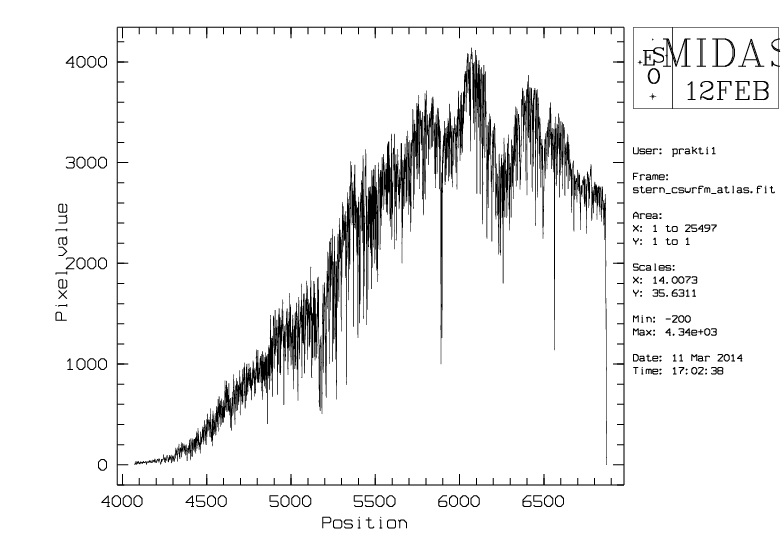
\includegraphics[height=.4\textheight]{images/stern_messung_spektrum.png}
\caption{Spektrum des beobachteten Sterns}
\label{fig:stern_messung_spektrum}
\end{figure}
In Abbildung \ref{fig:stern_messung_spektrum}, Seite \pageref{fig:stern_messung_spektrum} ist das Spektrum des beobachteten Sterns dargestellt. Es sind viele Linien zu erkennen, weswegen zu vermuten ist, dass der Stern zu den kalten Spektralklassen F,G,K und M gehört.
\\
\begin{figure}
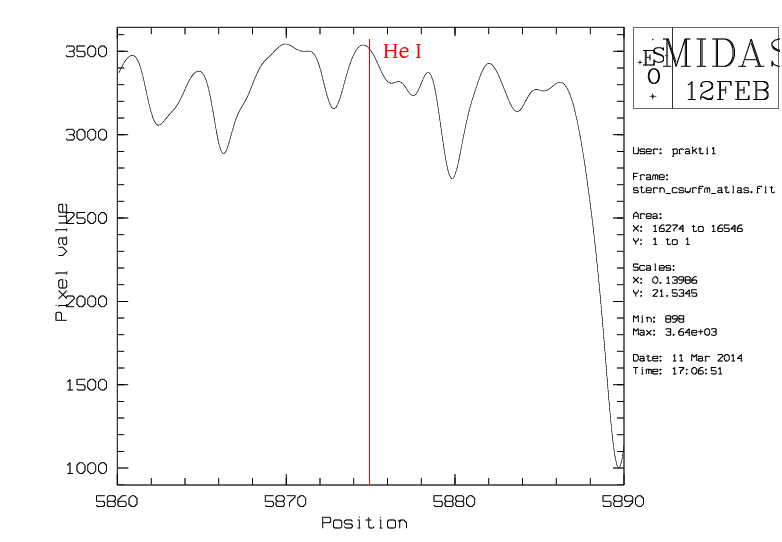
\includegraphics[height=.4\textheight]{images/stern_messung_HeI.png}
\caption{Mögliche Position der HeI-Linie im Spektrum des beobachteten Sterns}
\label{fig:stern_messung_HeI}
\end{figure}
Wie in Abbildung \ref{fig:stern_messung_HeI}, Seite \pageref{fig:stern_messung_HeI} zu erkennen, ist im Spektrum des beobachteten Sterns keine He I-Linie bei $5875.70 \AA$ identifizierbar, ein weiteres Indiz dafür, dass der Stern zu den kalten Spektralklassen gehört.
\\
\begin{figure}
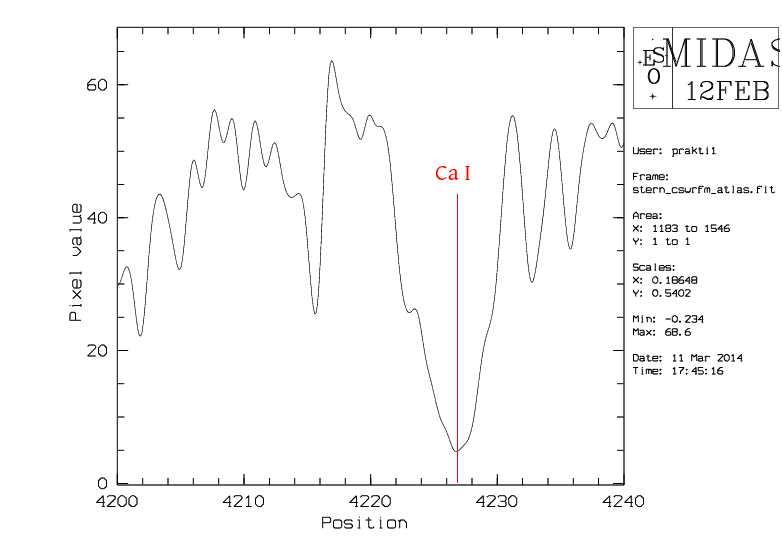
\includegraphics[height=.4\textheight]{images/stern_messung_CaI.png}
\caption{Position der CaI-Linie im Spektrum des beobachteten Sterns}
\label{fig:stern_messung_CaI}
\end{figure}
In Abbildung \ref{fig:stern_messung_CaI}, Seite \pageref{fig:stern_messung_CaI} ist die CaI-Linie bei $4226.74 \AA$ klar identifizierbar, also ist der Stern wahrscheinlich nicht in Klasse F.
\\
\begin{figure}
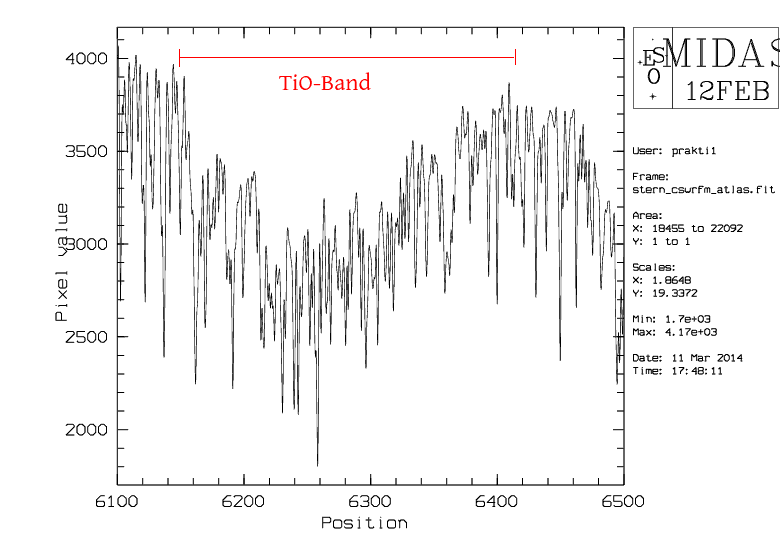
\includegraphics[height=.4\textheight]{images/stern_messung_TiO.png}
\caption{Position des TiO-Bands im Spektrum des beobachteten Sterns}
\label{fig:stern_messung_TiO}
\end{figure}
In Abbildung \ref{fig:stern_messung_TiO}, Seite \pageref{fig:stern_messung_TiO} ist das TiO-Band zwischen den Wellenlängen $6200 - 6400 \AA$ gut zu erkennen, welches nur in Klasse M-Sternen vorkommt.\
\\
Diese Indizien sprechen klar dafür, dass der beobachtete Stern in die Spektralklasse M einzuordnen ist.

\paragraph{Stern 2}
\begin{figure}
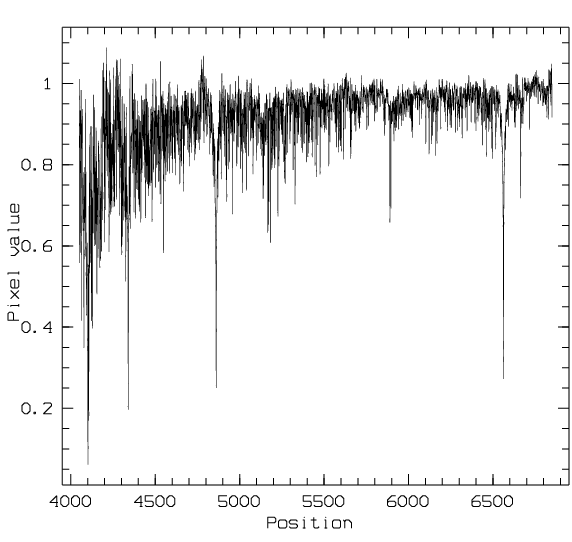
\includegraphics[height=.4\textheight]{images/stern2_spektrum.png}
\caption{Spektrum von Stern 2}
\label{fig:stern2_spektrum}
\end{figure}
Im Spektrum von Stern 2 (Abbildung \ref{fig:stern2_spektrum}, Seite \pageref{fig:stern2_spektrum}) sind viele Linien zu erkennen, was wiederum darauf schließen lässt, dass der Stern in die Klassen F,G,K oder M einzuordnen ist.
\\
\begin{figure}
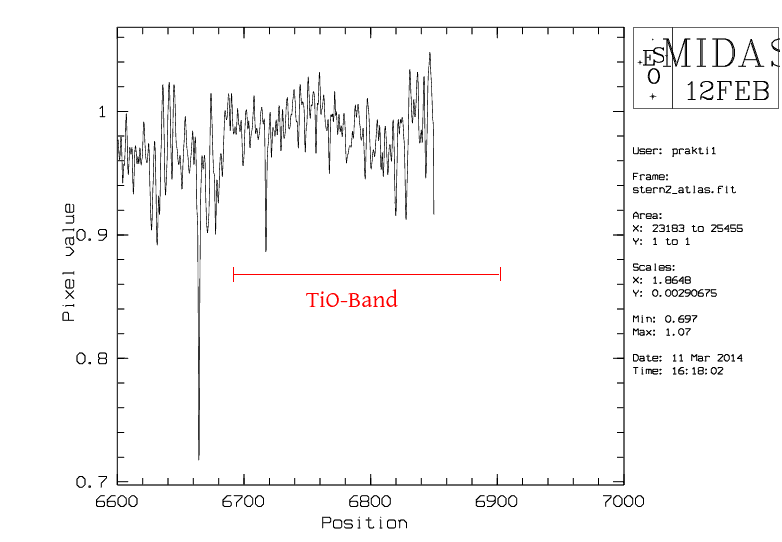
\includegraphics[height=.4\textheight]{images/stern2_TiO.png}
\caption{Mögliche Position des TiO-Bandes im Spektrum von Stern 2}
\label{fig:stern2_TiO}
\end{figure}
Zwischen den Wellenlängen $6700-7000 \AA$ ist kein TiO-Band zu erkennen, was eine Einteilung in Klasse M ausschließt.
\\
\begin{figure}
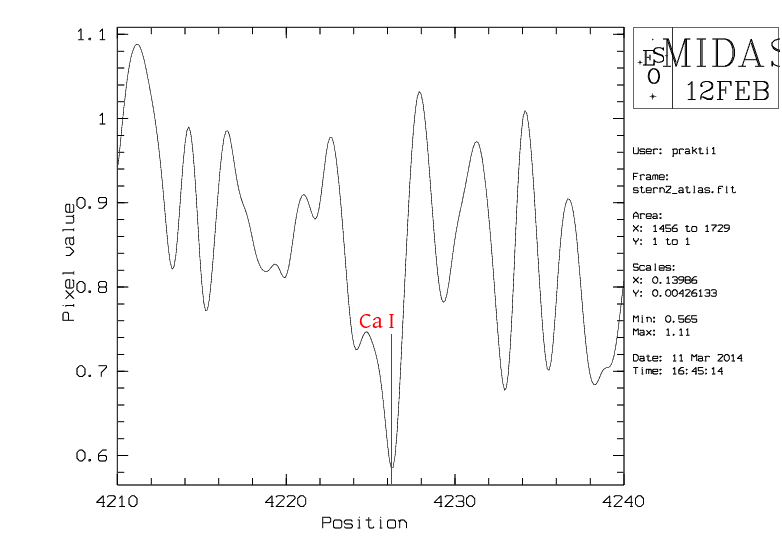
\includegraphics[height=.4\textheight]{images/stern2_CaI.png}
\caption{Position der CaI-Linie im Spektrum von Stern 2}
\label{fig:stern2_CaI}
\end{figure}
Bei der Wellenlänge $4226.74 \AA$ ist die CaI-Linie klar identifizierbar, weswegen der Stern nicht in die Klasse F eingeordnet werden kann.
\\
\begin{figure}
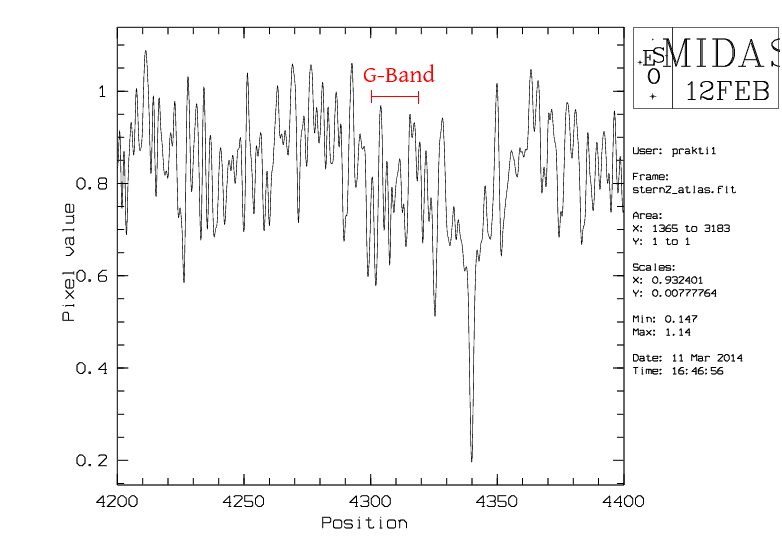
\includegraphics[height=.4\textheight]{images/stern2_G-Band.png}
\caption{Mögliche Position des G-Bandes im Spektrum von Stern 2}
\label{fig:stern2_CaI}
\end{figure}
In der Umgebung der Wellenlänge $4310 \AA$ ist kein G-Band zu erkennen, weshalb der Stern kein G-Stern sein kann.
\\
Damit bleibt nur noch die Klasse K als mögliche Einteilung übrig.

\paragraph{Stern 3}
\begin{figure}
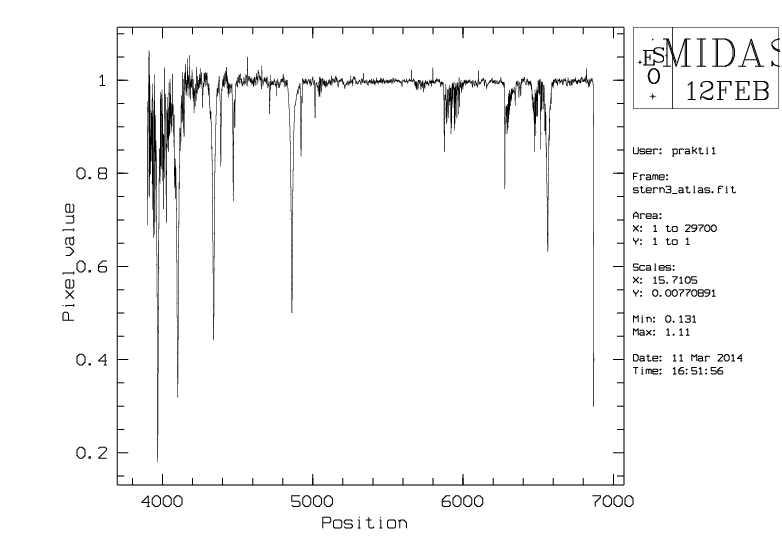
\includegraphics[height=.4\textheight]{images/stern3_spektrum.png}
\caption{Spektrum von Stern 3}
\label{fig:stern3_spektrum}
\end{figure}
Im Spektrum von Stern 3 (Abbildung \ref{fig:stern3_spektrum}, Seite \pageref{fig:stern3_spektrum}) sind wenige Linien mit einigen klar definierten Peaks zu erkennen. Daraus lässt sich schließen, dass der Stern in die heißen Spektralklassen O,B oder A  eingeordnet werden muss.

\begin{figure}
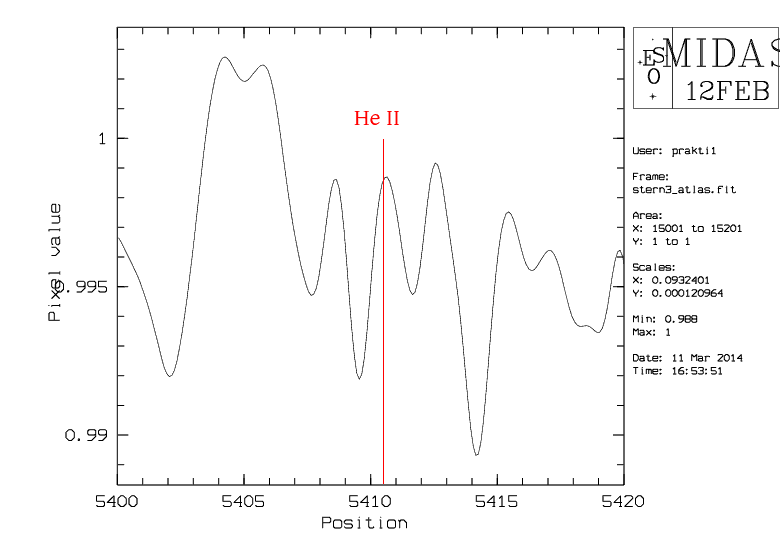
\includegraphics[height=.4\textheight]{images/stern3_HeII.png}
\caption{Mögliche Position der HeII-Linie im Spektrum von Stern 3}
\label{fig:stern3_HeII}
\end{figure}
Bei $5411.52 \AA$ ist keine HeII-Linie identifizierbar, der Stern kann also kein O-Stern sein.
\\
\begin{figure}
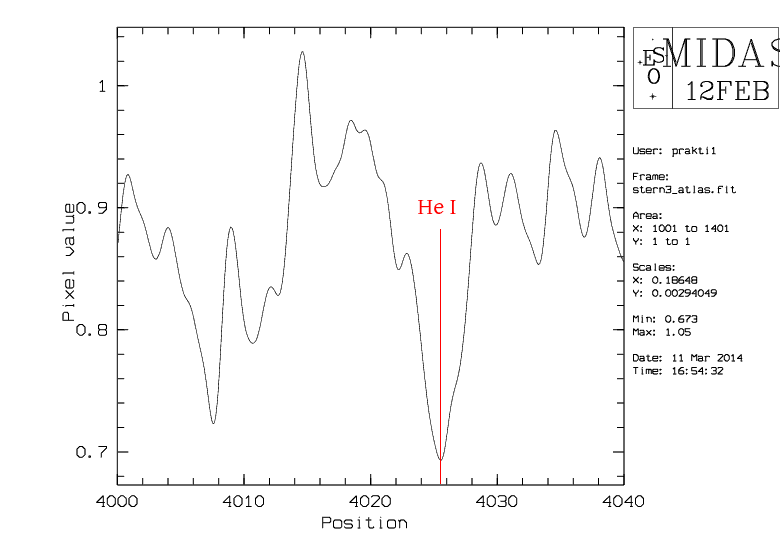
\includegraphics[height=.4\textheight]{images/stern3_HeI.png}
\caption{Position der HeI-Linie im Spektrum von Stern 3}
\label{fig:stern3_HeI}
\end{figure}
Die HeI-Linie bei $4026.20 \AA$ ist eindeutig erkennbar. Daraus lässt sich nun schließen, dass der Stern innerhalb der Spektralklasse B einzuordnen ist.

\newpage
\subsubsection{Bestimmung der Radialgeschwindigkeit}
Im Spektrum des gemessenen Sterns wurden mehrere Linien identifiziert und mit den theoretischen Wellenlängen verglichen, um die Dopplerverschiebung zu bestimmen. Hierbei sind alleinstehende und schmale Linien zu bevorzugen, weil sich durch die Verschiebung sonst Linien überlagern könnten.\
Die Geschwindigkeiten wurden mit der relativistischen Dopplerformel (die klassische Formel wäre auch ausreichend gewesen, hat jedoch zunächst absurde Ergebnisse geliefert, was evtl. an fehlerhafter Eingabe im Rechner lag)
\begin{equation}
f_B = f_Q \sqrt{\frac{c+v}{c-v}} \Leftrightarrow v = \frac{f_B^2 - f_Q^2}{f_B^2 + f_Q^2} \cdot c = \frac{\lambda_Q^2 - \lambda_B^2}{\lambda_B^2 + \lambda_Q^2}\cdot c
\end{equation}
wobei die Größen mit Index B für den Betrachter und Q für die Quelle stehen.\
Die Ergebnisse sind in Tabelle \ref{tab:Radial} dargestellt.

\begin{table}[htbp]
\begin{tabular}{c|c|c|c|c}
Element & theoretische Wellenlänge in $\AA$ & gemessene Wellenlänge in $\AA$ & $\Delta\lambda$ & V in km/s \\ \hline
Ca I & 4226.74 & 4226.685 & 0.055 & 3.90 \\ 
Fe I & 4383.56 & 4383.705 & -0.145 & -9.92 \\ 
Fe I & 5328.05 & 5328.087 & -0.037 & -2.10 \\ 
Ca I & 6162.18 & 6161.736 & 0.444 & 21.60 \\ 
Na I & 5889.97 & 5889.672 & 0.298 & 15.17 \\ 
Fe I & 4891.5 & 4890.983 & 0.517 & 31.70 \\ 
\end{tabular}
\caption{Bestimmung von Radialgeschwindigkeiten für den gemessenen Stern}
\label{tab:Radial}
\end{table}

Aus den berechneten Geschwindigkeiten lässt sich ein Mittelwert mit Standardabweichung berechnen, dies ist aber aus mehreren Gründen nicht sonderlich aussagekräftig. Der berechnete Wert wäre
\begin{equation}
\overline{v} = 10.1 \pm 15.6 \ \mathrm{km/s}
\end{equation}
Die Standardabweichung ist offensichtlich sehr groß, was vor allem daran liegt, dass nur wenige Linien ausgewertet wurden und der Fit in MIDAS auch nur begrenzte Genauigkeit hat. Vor allem treten sowohl positive als auch negative Verschiebungen auf, weswegen aus diesen Ergebnissen keine klare Erkenntnis gewonnen werden kann. 
Weiterhin muss gesagt werden, dass die Verschiebung sich aus mehreren Komponenten zusammensetzt, so bewegt sich nicht nur der Stern radial von der Erde weg, sondern auch die Sternwarte wegen der Erddrehung, die Erde bewegt sich um die Sonne, das Sonnensystem um das galaktische Zentrum und die Milchstraße relativ zur Galaxie des Sterns. Die Bestimmung der Geschwindigkeit des Sterns relativ zur Erde ist also nicht so einfach durchzuführen. 



\section{Fazit}
Abschließend lässt sich sagen, dass der Versuch sehr erfolgreich verlaufen ist. MIDAS hat sich als sehr effektives und relativ einfach zu bedienendes Werkzeug erwiesen, mit dem die Auswertung der Spektren gut möglich war. Die Einteilung der Sterne in Spektralklassen konnte anhalb weniger simpler Kriterien erfolgreich vorgenommen werden, eine genauere Einteilung in Unterklassen dürfte mittels einer genaueren Untersuchung möglich sein.\
Die Tatsache, dass selbst mittels der eher oberflächlichen Untersuchung des Spektrums wichtige Informationen über die Sterne gefunden werden konnten zeigt, wieso die Spektroskopie ein wichtiges Werkzeug der Astronomie ist.
\bibliographystyle{natdin}
\begin{thebibliography}{9}
%\bibitem[Bec]{kmann} BECKMANN, Dieter. Astrophysik. C.C.Buchner, 2011.
\bibitem[Spe]{ktroskopie} Wikipedia: Spektroskopie. Online im Internet: URL: http://de.wikipedia.org/wiki/Spektroskopie (Stand: 11.03.2014). 
\bibitem[Ast]{ronomischesPraktikum} Astronomisches Praktikum.
\end{thebibliography}

\newpage
%\bibliographystyle{natdin}
%\bibliography{literature}
\section{Anhang}

\begin{table}[h!]
\centering
\begin{tabular}{c|c|c|c}
Winkel Sonne & Zwischenzeit (h min s) & Endzeit (h min s) & MEZ Funkuhr \\ 
\hline 
180 $^\circ$  13' 54'' & $2^m 16.18^s$  & $2^m 59.18^s$ & $10^h 52^m 00^s$ \\ 

182 $^\circ$  29' 01'' & $2^m 14.44^s$  & $3^m 00.03^s$ & $10^h 59^m 30^s$ \\ 

183 $^\circ$  37' 44'' & $2^m 14.18^s$  & $2^m 44.53^s$ & $11^h 03^m 00^s$ \\ 

184 $^\circ$  50' 08'' & $2^m 13.75^s$  & $2^m 48.85^s$ & $11^h 07^m 00^s$ \\ 

189 $^\circ$  03' 04'' & $2^m 12.44^s$  & $2^m 48.78^s$ & $11^h 20^m 30^s$ \\ 

190 $^\circ$  13' 49'' & $2^m 11.83^s$  & $3^m 05.00^s$ & $11^h 24^m 30^s$ \\ 

191 $^\circ$  45' 55'' & $2^m 11.68^s$  & $3^m 16.66^s$ & $11^h 29^m 30^s$ \\ 

193 $^\circ$  07' 52'' & $2^m 11.00^s$  & $2^m 31.37^s$ & $11^h 33^m 00^s$ \\

\end{tabular} 
\label{tab:sun}
\caption{Messung des Sonnenazimut}
\end{table}

\begin{table}[h!]
\centering
\begin{tabular}{c}

Gemessener Azimut \\
\hline
117 $^\circ$ 40' 24'' \\ 

117 $^\circ$ 40' 24'' \\ 

117 $^\circ$ 40' 22'' \\ 

117 $^\circ$ 40' 23'' \\ 

117 $^\circ$ 40' 24'' \\ 

117 $^\circ$ 40' 22'' \\ 

117 $^\circ$ 40' 24'' \\ 

117 $^\circ$ 40' 22'' \\ 

\end{tabular}
\caption{Messung des Turmazimut}
\label{mess_turm}
\end{table}


\begin{table}[h!]
\centering
\begin{tabular}{c}
Berechneter Sonnenazimut \\
\hline
330.207231345\\
332.460255182\\
333.606001818\\
334.812139975\\
339.025513227\\
340.206071994\\
341.739111616\\
343.104060402\\
\end{tabular}
\caption{Berechneter Sonnenazimut}
\label{sonnenaz}
\end{table}

\end{document}